In this chapter we investigate the consequences of two nonlinear parameters which are the   \textbf{steepness} $\varepsilon_1= k a$, and the amplitude normalized by the water depth $\varepsilon_2= a/D$. 
The linear theory of \ref{ch1b} was obtained in the limit of $\varepsilon_1=0$ and $\varepsilon_2=0$. After giving the full equations for nonlinear wave motion, this chapter focuses on the properties 
of monochromatic waves. The next chapter will consider the solution up to second order in $\varepsilon_1$ but extended to a random wave field. 



\section{Dimensional analysis and importance of $\varepsilon_1$ and $\varepsilon_2$ }
In order to simplify the equations, we will assume here that the mean water level is  $\overline{\zeta}=0$, so that the mean water depth is  $D=h$. 

The wave equation for irrotational waves includes non-linear terms in addition to the linear term given in chapter \ref{ch1b}. These come from the 
advection in the momentum equation or $u^2$ and $w^2$ terms in the Bernoulli equation,  
\begin{equation}
    \frac{\partial \phi}{\partial t}=
    -\frac{1}{2}\left[
    \left|\bnabla \phi\right|^2
    +\left(\frac{\partial \phi}{\partial z}\right)^2
    \right]
    -\frac{p}{\rho_w}-g z + C(t),\label{Bernoulli_nl}
\end{equation}

and the surface kinematic boundary condition, 

\begin{equation}
    w=\frac{\partial \phi }{\partial z}= {\mathbf u}\bcdot \bnabla \zeta + \frac{\partial \zeta }{\partial t}= \bnabla {\mathbf \phi}\bcdot\bnabla \zeta
    + \frac{\partial \zeta }{\partial t}
    \quad \mbox{sur\ }\quad z=\zeta.  \label{eq:surface_nl}
\end{equation}

Taking $\partial (\ref{Bernoulli_nl} \textrm{~at~z=}\zeta)/\partial t $
+$g\times$(\ref{eq:surface_nl}) in order to eliminate the linear $\zeta$ terms, gives \footnote{Be careful that, when computing 
$\partial (\ref{Bernoulli_nl})/\partial t$ at $z=\zeta$, you should not forget that  $\zeta$ is a function of time.}
\begin{equation}
  \frac{\partial^2{\phi}}{\partial{t^2}}+g\frac{\partial\phi}{\partial z}=
g\bnabla\phi \cdot \bnabla\zeta - \frac{1}{2}\frac{\partial \zeta}{\partial
t}\frac{\partial^2 \phi}{\partial z \partial t}-  \frac{1}{2} \left(\frac{\partial }{\partial t}+\frac{\partial
\zeta}{\partial t}\frac{\partial }{\partial z}\right) \left[\bnabla\phi \cdot
{\bnabla\phi} + \left(\frac{\partial\phi}{\partial
z}\right)^2\right]+C'(t), \quad \mbox{at}
\quad  z=\zeta. \label{surface comb}
\end{equation}

We note that the non-linearity comes from the terms on the right hand side but also from the fact that  eq. (\ref{surface comb}) 
is valid  at $z=\zeta$, which is unknown. Indeed,  a Taylor expansion around $z=0$ adds many terms, for example 
\begin{equation}
\left. \frac{\partial^2{\phi}}{\partial{t^2}} \right|_{z=\zeta} \simeq \left. \frac{\partial^2{\phi}}{\partial{t^2}} + \zeta \frac{\partial^3{\phi}}{\partial{t^2} \partial z}  
+ \frac{1}{2}\zeta^2 \frac{\partial^4{\phi}}{\partial{t^2} \partial z^2} + ...  \right|_{z=0}
\end{equation}


Before solving this, a question arises: should we really keep all these terms? Do they have the same importance?  This is where a dimensional 
analysis of  eq. (\ref{surface comb}) is necessary. This requires to define scales for time and space. 

Because we are studying waves, they are naturally characterized by a wavelength  $L=2 \upi/k$, a period $T$, and their amplitude $a$. 
Besides, the water depth  $D=h+\overline{\zeta}$
comes in the bottom boundary condition. Finally, gravity 
$g$ is constant and naturally links space and time scale. We can recall the Reech-Froude law for hydrodynamics: if time is multiplied by  $\alpha$,
then space is multiplied by  $\alpha^2$, and velocities by  $\alpha$.

We can thus consider that the time scale is fixed by the spatial scale and our problem is thus only a function of the 
ratios of the different space scales. Since we have  $a$, $k$ et $D$, we can make two independent ratios which can be  $\varepsilon_1= k a$,
 $\varepsilon_2= a/D$, or $\mu=kD$. The combination of the last two gives the \cite{Ursell1953} number  
 \begin{equation}
\Ur=\varepsilon_2/\mu^2
 \end{equation}
It is common to use  $\varepsilon_1$ and
$\mathrm{Ur}$. We will see below that a Froude number $\alpha=g a /
C^2$, where $C$ is the phase speed, can also have interesting properties \citep{Kirby1998}.

Let us now look at the different terms in eq. (\ref{surface comb})
 following the analysis of \cite{Kirby1998}. We take 
 \begin{eqnarray}
  x'&=&k_0 x, \\
  y'&=& k_0 y, \\
  t'&=&k_0 C_0 t, \\
  \zeta'&=&\zeta/a.
 \end{eqnarray}
 This gives  $\phi'=\phi/\phi_0$
where $\phi_0= C \alpha /k$ and the Froude number is 
 \begin{equation}
\alpha=g a / C^2.
 \end{equation}
For the vertical coordinate we choose a scale  $Z$, giving $z'=z/Z$. 
Eq. (\ref{surface comb}) thus becomes 
\begin{eqnarray}
   \frac{\partial^2{\phi'}}{\partial{t'^2}}&+&\frac{g}{Z k_0^2 C_0^2} \frac{\partial\phi'}{\partial
   z'}=
\alpha  \bnabla\phi' \cdot \bnabla\zeta' - \frac{a}{Z} \frac{\partial
\zeta'}{\partial t'}\frac{\partial^2 \phi'}{\partial z' \partial t'}
\nonumber\\
& &- \left(1+\frac{akC}{Z} \frac{\partial \zeta'}{\partial t'}\frac{\partial
}{\partial z'}\right) \alpha \left[\bnabla\phi' \cdot
\frac{\partial{\bnabla\phi'}}{\partial t'} + \frac{1}{k_0^2 Z^2}
\frac{\partial\phi'}{\partial z'}\frac{\partial^2\phi'}{\partial t'\partial
z'}\right]+\frac{C'(t)}{\phi_0 k_0^2 C_0^2}, \quad \mbox{at} \quad
z'=\frac{a}{Z}\zeta'. \nonumber\\ \label{surface comb_scale}
\end{eqnarray}

If one chooses $Z=1/k$, then $\alpha=a/Z=\varepsilon_1$ and the linear wave equation only requires  $\varepsilon_1 \ll 1$. Choosing instead $Z=D$, will also require $\varepsilon_2=a/D \ll 1$. 
Hence the linear wave theory requires both $\varepsilon_1 \ll 1$  and $\varepsilon_2 \ll 1$. It is easy to verify that the solution given in chapter \ref{ch1b} 
are indeed consistent with these assumptions.




\section{Finite amplitude solutions}\label{ch_nonlin_per}
\subsection{Stokes expansion for weak non-linearity}
The common method, introduced by \cite{Stokes1880} is to expand the solution to the nonlinear equations in 
powers of $\varepsilon_1$, which is most appropriate for deep water waves, 
\begin{eqnarray}
\phi &=& \phi_{1}+  \phi_{2}+ \phi_{3}
    +..., \\
    \zeta &=& \zeta _{1}+ \zeta_{2}+ \zeta_{3}
    + ...,
    \label{power expansion}
\end{eqnarray}
in which each term of index $n$ is of order $\varepsilon^n$.
\cite{Levi-Civita1925} proved that this expansion was convergent for monochromatic waves. For general random waves, 
$\phi _{1}$ is the solution to the linear equations  (\ref{surface 1}), and thus  $\phi_1$ is a 
linear sum of monochromatic waves as determined in chapter \ref{ch1b},
\begin{equation}
    \phi _{1}=\sum_{\kb,s}\frac{\cosh \left( k z+k h\right) }{\cosh \left( kh\right) }
    \Phi _{1,\kb}^{s}\left(\skew4\widetilde{t} \; \right) \mathrm{e}^{\mathrm{i}
    \left(\kb\bcdot{\mathbf x} - s \sigma t\right)},
  \label{phi}
\end{equation}
where $\sigma$ and $\kb$ are related by the linear dispersion relation (\ref{dispersion}). 

Tke long term evolution of the amplitudes $\Phi
_{1,\kb}^{s}$ on time scales
$\skew4\widetilde{t} \;$ is not constrained by the linear equations which give constant amplitudes, but this evolution 
will be part of the solution at higher orders. 

When we collect all terms of second order, we have a wave equation for  $\phi_2$, which is forced by products of $\phi_1$ and $\zeta_1$. The full 
second order solution is given in chapter \ref{chnl2}. 


We also note that at third order, one obtains a modification of the phase speed. For monochromatic waves in deep water 
this is \citep{Stokes1880}
\begin{equation}
    C=gk \left[1+ k^2 a^2\right].
\end{equation}


Stokes waves are generally unstable any small perturbation will grow to produce shorter and longer components that will exchange 
energy with the initial wave. This is known as the instability of
\cite{Benjamin&Feir1967}. Finite amplitude growth was further analyzed by \cite{Chalikov2007}. 
%Ainsi la houle de Stokes n'existe pas en réalité. Pour $ak
%> 0.13$ certaines des vagues irrégulières issues de l'instabilité
%évoluent vers des formes toujours plus cambrées jusqu'à déferler.

\subsection{Numerical methods for finite amplitude periodic waves}
The analytical calculation of the amplitude of different harmonics is becomes very tedious at higher order and has only been completed 
up to fifth order by \cite{De1955}. Beyond fifth order, several method can provide very accurate numerical solutions \citep{Dean1965,Dalrymple1974,Schwartz1974}. 
Such methods have been used by \cite{Longuet-Higgins&Fenton1974} to show that energy and phase speed first grow and then decrease as the wave height increases. Hence, the 

Here we use the streamfunction method of Dean, as extended by Dalrymple to allow for a linear current shear such that the velocity potential still 
satisfies Laplace's equation. This iterative method fits the Fourier amplitudes of the velocity potential to minimise the deviations from a constant pressure 
along the sea surface. This easily produces the first 100 harmonics for waves that can be really steep, with  orbital velocities at the crest 
$u_{\mathrm{max}}$ up to  98\% of the phase speed  $C$, as shown in figure \ref{Fig_amplitude_finie}. 
We recall that periodic waves break when 100\% is reached and no periodic waves can exist with orbital velocities 
%Lorsque $u_{\mathrm{max}}$
%s'approche de $C$, en particulier pour les faibles profondeurs $kD
%< 0.3$, la convergence vers la solution devient plus délicate.
These near-breaking waves are particularly interesting for exploring the kinematics and energetics of breaking waves, although 
real breaking waves can be very different due to their non-stationary shapes. 
\cite{Cokelet1977}) introduced the small parameter 
\begin{equation}
    \epsilon = \left[1 - \frac{q_{\mathrm{crest}}^2
    q_{\mathrm{trough}}^2}{C^4}\right]^{1/2}
\end{equation}
with $q_{\mathrm{crest}}$ and $q_{\mathrm{trough}}$ the orbital velocities at the crest and trough in the frame 
of reference moving with the wave, so that $q_{\mathrm{crest}}=u_{\mathrm{max}}-C=0$ in the case of nearly breaking wave. 
This parameter is clearly between 0 et 1 and allows an expansion in powers of  $\epsilon$ for nearly breaking waves. 


\subsection{Kinematics of finite amplitude waves}
Finite amplitude waves are characterized by flat trough and steeper crests, in particular in shallow water. The orbital 
velocities are even more asymetric with much larger velocities at the crest than in the troughs. At the limit 
when $u_{\mathrm{max}}/C = 1$ the surface slope is discontinuous with a  $120^\circ$  angle at the crest. 
%%%%%%%%%%%%%%%%%%%%%%%%%%%%%%%%%%%%%%%%%%%%%%%%%%%%%%%%%%%%%%%%%%%%%%%%%%%%
\begin{figure}[htb]
\centerline{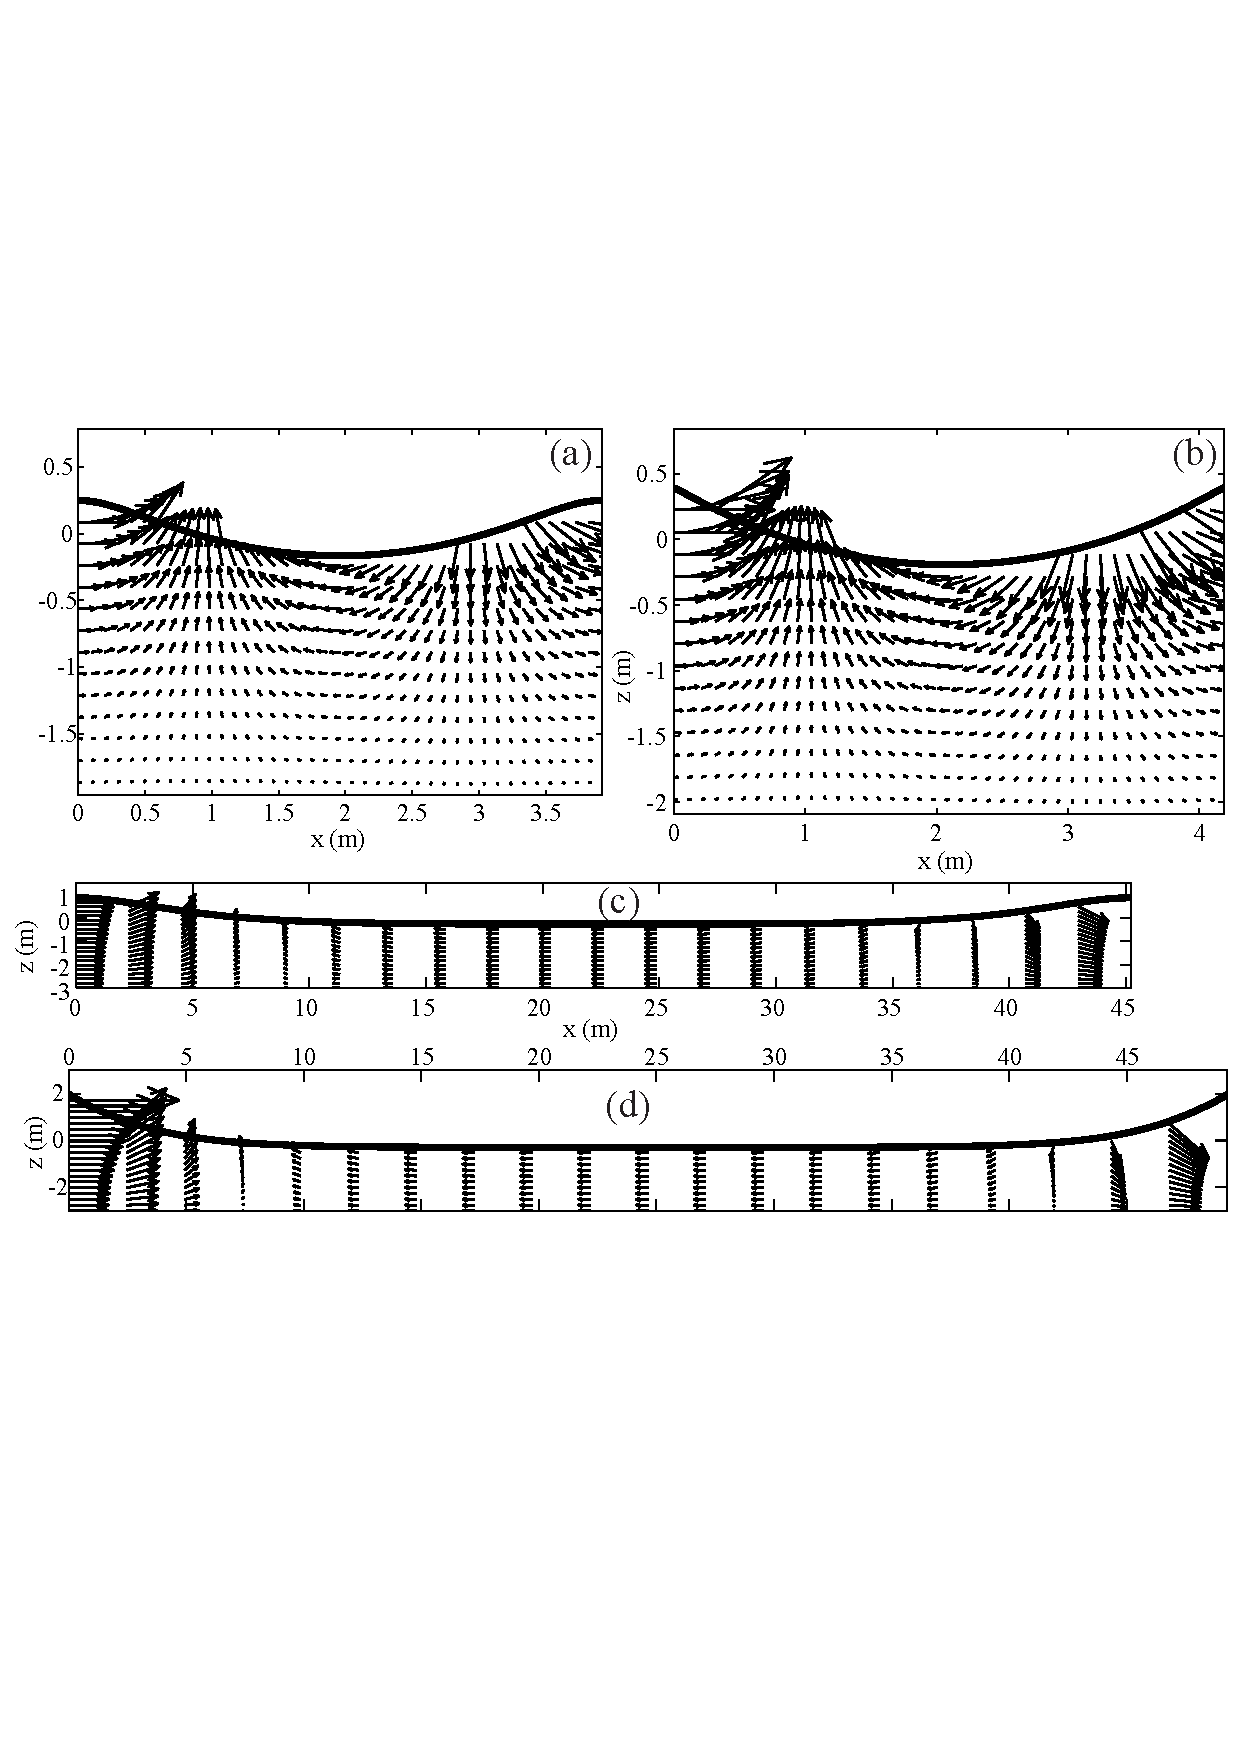
\includegraphics[width=0.9\textwidth]{FIGURES/vagues_amplitude_finie.pdf}}
%\vspace{3.64in}
\caption{Surface elevations and velocity fields at 60th order using \cite{Dalrymple1974}'s numerical method 
for a water depth of 3 m. (a) and (b) are deep water  waves with a period of 1.5~s, so that  $kD\simeq 5$.  
(c) and (d) are shallow water waves of 8~s period. The nonlinearity is intermediate for (a) and (c), with $u_{\mathrm{max}}/C\simeq 0.3$, 
and extreme in (b) and (d)  with $u_{\mathrm{max}}/C\simeq 0.97$.}
\label{Fig_amplitude_finie}
\end{figure}
%%%%%%%%%%%%%%%%%%%%%%%%%%%%%%%%%%%%%%%%%%%%%%%%%%%%%%%%%%%%%%%%%%%%%%%%%%%%

These nonlinear effects have several consequences. In particular the phase speed, energy and Stokes drift are slightly higher (up to 10\% in deep water, much more in shallow water) than predicted 
by linear theory with the same surface elevation variance  \citep{Cokelet1977}. If accurate estimations of wave kinematics are needed, the linear theory may 
not be good enough. To know how far the nonlinear solution differ from the linear theory, it is possible to compute numerically the finite amplitude solutions. 
For example, in the shallow water limit, the surface Stokes drift can exceed several times the linear value \citep{Ardhuin&al.2008}.



\subsection{Integral properties}
The properties of periodic finite amplitude waves over a flat bottom still follow some exact relations. Here we reproduce the results of  \citep{Cokelet1977}. For any water level  $z_0$ below the wave troughs (i.e. such that  $-h <z_0 < \min(\zeta)$) we may define, 
\begin{eqnarray}
\mathcal{M}&=&\frac{1}{L}\int_0^{L} \rho_w \zeta {\mathrm d}x =
\rho_w \overline{\zeta}, \\
\mathcal{C}&=&\frac{1}{L}\int_0^{L} \rho_w u(x,z_0) {\mathrm d}x =
\rho_w \overline{u}, \\
M^w&=&\overline{\int_{-h}^{\zeta} \rho_w u {\mathrm d}z}, \\
E_c&=&\frac{1}{2}\overline{\int_{-h}^{\zeta} \rho_w \left(u^2+w^2\right) {\mathrm d}z}, \\
E_p&=& \overline{\int_{\overline{\zeta}}^{\zeta} \rho_w g z  {\mathrm d}z}, \\
S_{xx}&=&\overline{\int_{-h}^{\zeta} \left(p + \rho_w u^2\right)
{\mathrm d}z} -\overline{\int_{-h}^{\zeta} p^H {\mathrm d}z} =
\overline{\int_{-h}^{\zeta} \left(p + \rho_w u^2\right) {\mathrm
d}z} - \frac{1}{2} \rho_w g D^2, \\
F&=&\overline{\int_{-h}^{\zeta} \left[p + \frac{1}{2}\rho_w
\left(u^2+w^2\right)+\rho_w g \left(z-_zeta\right) \right] u
{\mathrm
d}z},\\
\overline{u_b^2}&=&\frac{1}{L}\int_0^{L} u^2\left(x,-h,t\right)
{\mathrm d}x.
\end{eqnarray}

In the frame of reference moving at the phase speed, the following three quantities are are independent of the horizontal position  $x$. These are 
the mass flux per unit crest length, 
\begin{equation}
-Q=\int_{-h}^{\zeta} \rho_w \left(u-C\right) {\mathrm d}z = - \rho_w C d .
\end{equation}
%The depth scale  $d$ is such that a permanent flow of speed $C$ and with a mass flux equal to that induced by waves.
%A flow over depth $d$ that would have the same mass transport would have a speed 
%\begin{equation}
%c_m=-\overline{\frac{1}{d+\zeta}\int_{-h}^{\zeta} u-C {\mathrm
%d}z} = C d/D.
%\end{equation}
the dynamic pressure 
\begin{equation}
R=\frac{p}{\rho_w g} +
\frac{1}{2g}\left[\left(u-C\right)^2+w^2\right]+\left(z+h\right),
\end{equation}
and the momentum flux per unit crest length 
\begin{equation}
S=\int_{-h}^{\zeta}\left[p+\left(u-C\right)^2\right]{\mathrm d}z.
\end{equation}

These quantities are used in other relations 
\begin{eqnarray}
M^w&=&\rho_w C D - Q, \\
2 E_c &=& C M^w - \rho_w \mathcal{C} , \\
S_{xx}&=&4 E_c - 3 E_p+\rho_w \overline{u_b^2}+\rho_w C^2 \\
F&=& C \left(3 E_c - 2 E_p\right)+\frac{1}{2}
\overline{u_b^2}\left(M^w+\rho_w C D\right) + C\mathcal{C}Q \\
K&=&2 \frac{\mathcal{M}}{\rho_w}+\overline{u_b^2}+C^2, \\
R&=&\frac{1}{2}K + h, \\
S&=&S_{xx}-2C M^w +D \left(C^2+\frac{1}{2}D\right),
\end{eqnarray}
where $K$ is Bernoulli's constant, linked to the surface dynamic boundary condition of constant pressure along the sea surface,
\begin{equation}
K=\left(u-C\right)+w^2 + 2 \zeta \quad \mathrm{pour} \quad
z=\zeta
\end{equation}

\subsection{Nonlinear corrections to Airy waves}
Using periodic numerical solutions, one may propose empirical corrections for various quantities. For example, 
figure \ref{Mwfig} shows the expected correction for the wave momentum $M_w$, as a function of the  parameters $H/D$  and $kD$.

%%%%%%%%%%%%%%%%%%%%%%%%%%%%%%%%%%%%%%%%%%%%%%%%%%%%%%%%%%%%%%%%%%%%%%%%%%%%
\begin{figure}
\centerline{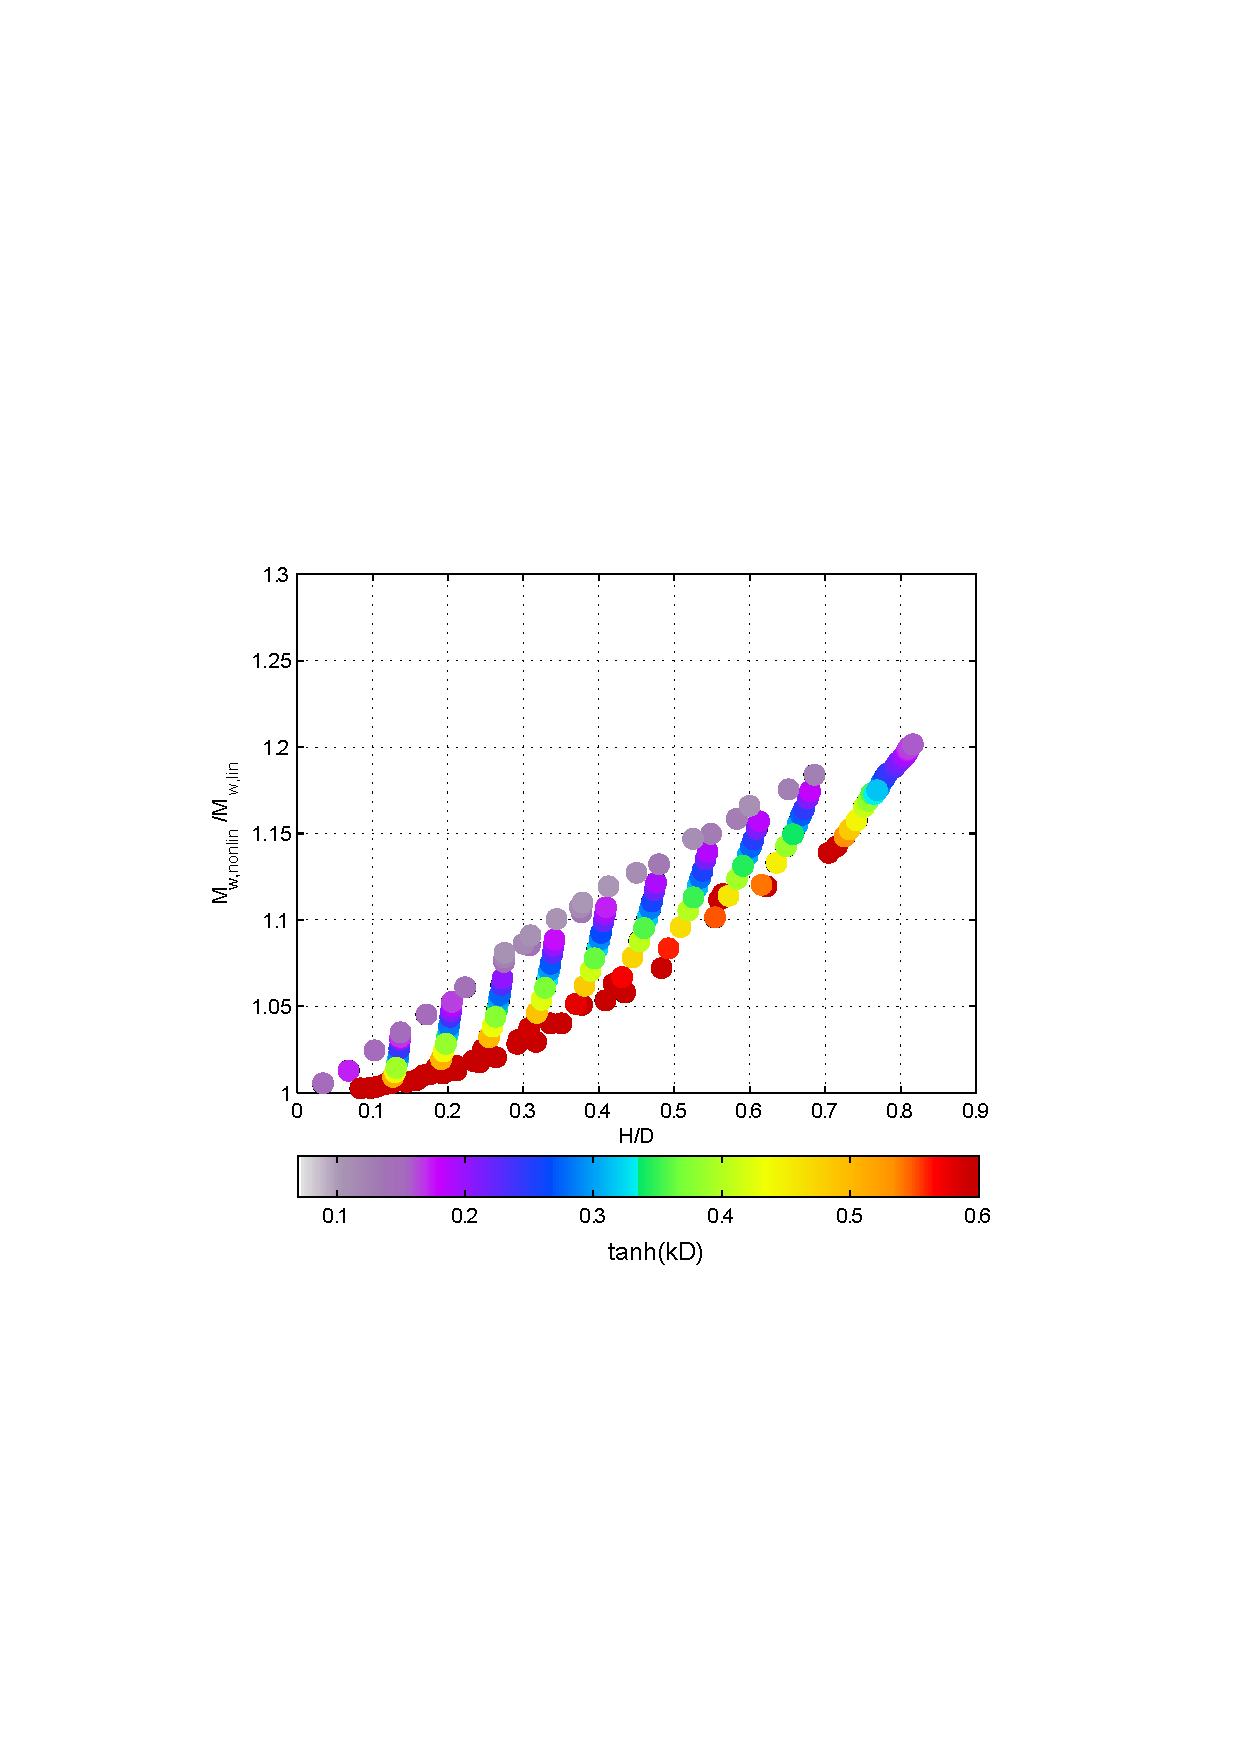
\includegraphics[width=0.6\textwidth]{FIGURES/MW_Mwlin.pdf}}
%\vspace{3.64in}
\caption{Ratio of the wave momentum for periodic waves of finite amplitude and linear waves with the same surface elevation variance. This was computed 
using the streamfunction theory of Dean and \cite{Dalrymple1974} with orders 80 to 120.} \label{Mwfig}
\end{figure}
%%%%%%%%%%%%%%%%%%%%%%%%%%%%%%%%%%%%%%%%%%%%%%%%%%%%%%%%%%%%%%%%%%%%%%%%%%%%


%ajouter un commentaire sur la conjecture de Benjamin-Lighthill (Benjamin 1995)
%\section{Houles non-stationnaires d'amplitude finie}


\section{Nonlinear theory for random waves}\label{ch_nonlin_alea}
Nonlinearity of random waves has a few distinct effects on the wave spectrum. First of all, the exchange of
energy between different spectral components is given by the  \cite{Hasselmann1960} theory, as introduced 
in chapter \ref{ch_evol_profond}.

\subsection{Dispersion relation}
Another effect is a change in the dispersion relation. That is particularly important when measuring currents 
using the dispersion relation, with a HF radar, or sequences or radar or optical images. \cite{Barrick&Weber1977} showed that for the wavenumber 
$k_B$ and wave direction $\theta_B$, a first correction of the deep water wave dispersion is  \citep{Broche&al.1983,Ardhuin&al.2008}, 
\begin{equation}
C_{2}(k_B,\theta_B) =  \frac{\sqrt{g}}{2} k_B^{3/2}
\int_{0}^\infty \int_0^{2 \pi} F(x,\alpha) E(f,\theta) \mathrm{d}
\theta \mathrm{d} f,\nonumber  \label{UsfA2}
\end{equation}
where, using
$y=x^{1/2}=f/f_B$ and $a=\cos \alpha$, 
\begin{equation}
F(x,\alpha)=y\left\{2 a - y+3 x a \right\} + y \sum_{\varepsilon=\pm 1} \frac{\varepsilon -a}{a_\varepsilon
- \left(1 +\varepsilon y\right)^2} \left\{\left(y a -x\right)\frac{a_\varepsilon+\left(1+\varepsilon
y\right)^2}{2} +\left(1+ \varepsilon y\right) \left(1+\varepsilon x a +
\varepsilon y\left(x+\varepsilon
a\right)-a_\varepsilon\right)\right\},
\label{A1corr}
\end{equation}
where
\begin{equation}
a_\varepsilon=\left(1+x^2 + 2 \varepsilon x a \right)^{1/2}.
\end{equation}
For $x<1$,  $F(x,0)=4
x^{3/2}$, and for $x>1$, $F(x,0)=4 x^{1/2}$ \citep{Longuet-Higgins&Phillips1962}. 
In general 
$F(x,\alpha)\simeq F(x,0) \cos \alpha$, with 	approximation errors under 5 \%. 
%  $x=1$, où  
%$F(x,\alpha) > F(x,0) \cos \alpha$ pour 
%$| \alpha | < \pi/3$, ce qui peut donner une erreur de 
%2 to 5\% par rapport à l'approximation  $F(x,\alpha)\simeq F(x,0) \cos \alpha$.

\subsection{Harmonics}\label{random_harmonics}
The presence of harmonics for random waves is a generalization of the harmonics for periodic waves. 
A first approximation, at second order, gives the harmonic corrections as a sum of interactions of the first order waves. However, to be complete in terms of spectrum, one needs to include not only the $\Phi_{2,2}^2 (\kb)$ terms that are the products of linear waves  $\Phi_1^2 (\kpb) \Phi_1^2 (\kb -\kpb)$, but also the interactions of third order with first order $\Phi_{3,1}(\kb) \Phi_{1,1} (\kb)$ avec $\Phi_{3,1}(\kb)$. These were typically note included by \cite{Weber&Barrick1977}. 

This omission is corrected in \cite{Creamer&al.1989} and \cite{Janssen2009}. That latter approach is well suited for numerical wave modelling: the wave amplitude variables are transformed following  \cite{Krasitskii1994} to remove resonances at second order: one can then compute the evolution of the transformed wave field and then the evolved field can be transformed back to "natural variables", which is a bit like adding the second order spectrum.
This approach has been particularly used to compute forces excerted by waves on structures 
\citep{Prevosto&Forristall2002}. 
% mais aussi pour la zone littorale où cela peut permettre de prendre en compte une bonne partie  de la génération des harmoniques. 

%Il semble que la théorie n'est pas encore tout à fait au point pour appliquer cette méthode dans des conditions de profondeur et courant variable, mais elle suggère une alternative interessante au calcul (faux) des interactions de 3 vagues  dans les modèles à phase moyennée. 

\section{Non-linear 4-wave interactions}
\subsection{Deep water evolution}
For a continuous wave spectrum, we find resonances that look like the forced oscillator solution in the case of the wind-generation in eq. (\ref{singularity}). 
For evolution times much longer than the wave period, the sixth order energy term that comes from third order amplitudes 
\begin{equation}
E_{3,3}(\kb)=\frac{|\dr Z_3(\kb)|^2 + |\dr \Phi_3(\kb)|^2}{2 \dr \kb}
\end{equation}
gives an evolution equation similar to eq. (\ref{croissance_lin})
\begin{equation}
\frac{\partial E_{3,3}(\kb) \left(\kb \right)}{\partial t} = \frac{\pi}{2}  \int |B|^2 E(\kb_1) E (\kb_2) 
E (\kb_3){\mathrm d}\kb_1{\mathrm d}\kb_2{\mathrm d}\kb_3.\label{E33}
\end{equation}

We can thus obtain the rate of change of the spectrum, 
\begin{equation}
 E(\kb)=E_2(\kb) + E_4(\kb) + E_6(\kb) + ...
\end{equation}
where we have left out the odd order terms (third order, fifth order) that are exactly zero in the case of a Gaussian sea state \citep{Hasselmann1962}.
We already know the second order terms, 
\begin{equation}
E_2(\kb)=2 \frac{|\dr Z_1(\kb,+)|^2}{\dr \kb} 
\end{equation}
and at 4th order the energy is not equally split between potential and kinetic energy so we have to add these two separately, 
\begin{equation}
 E_4(\kb)=\frac{1}{2 \dr \kb}\left\{\overline{|\dr Z_2(\kb)|^2} + 2 \Re\left[\overline{Z_1(-\kb) Z_3(\kb)}\right]
+ \frac{\sigma^2}{g^2}\overline{|\dr \Phi_2(\kb)|^2} + 2 \frac{\sigma^2}{g^2}\Re\left[\overline{\Phi_1(-\kb) \Phi_3(\kb)}\right] \right\}
\end{equation}
and we now have the 6th order term that have a long-term evolution, 
\begin{eqnarray}
 E_6(\kb)&=&\frac{1}{2 \dr \kb}\left\{\overline{|\dr Z_3(\kb)|^2} + 2 \Re\left[\overline{Z_1(-\kb) Z_5(\kb)}\right] + 
2 \Re\left[\overline{Z_2(-\kb) Z_4(\kb)}\right] \right. \nonumber \\
& &\left.
+ \frac{\sigma^2}{g^2}\overline{|\dr \Phi_3(\kb)|^2} + 2 \frac{\sigma^2}{g^2}\Re\left[\overline{\Phi_1(-\kb) \Phi_5(\kb)}\right] 
+ 2 \frac{\sigma^2}{g^2}\Re\left[\overline{\Phi_2(-\kb) \Phi_4(\kb)}\right] \right\}\label{E6}
\end{eqnarray}
This means that to do this right, one has to carry out the calculations of the amplitudes to 5th order, which was first done by \cite{Hasselmann1962}.

\subsection{4-wave interactions in shallow water}
As the water depth goes down, the interactions change shape because the wave kinematics and dispersion relation change. \citep{Janssen&Onorato2007} have shown that the previously proposed use of a DIA approximation with a coupling coefficient varying as a function of $kD$  may not work so well. 
Indeed the coupling coefficient $T$ for $k_1=k_2=k_3=k_4$ goes to zero at the depth $kD=1.363$, and is much weaker than in deep water when $1.2 < kD < 3$, as shown in Fig. 
\ref{T2_Snl_vs_KD}). There is still much debate on how to properly represent finite depth effects on 4-wave interactions. 
%%%%%%%%%%%%%%%%%%%%%%%%%%%%%%%%%%%%%%%%%%%%%%%%%%%%%%%%%%%%%%%%% figure
\begin{figure}
\centerline{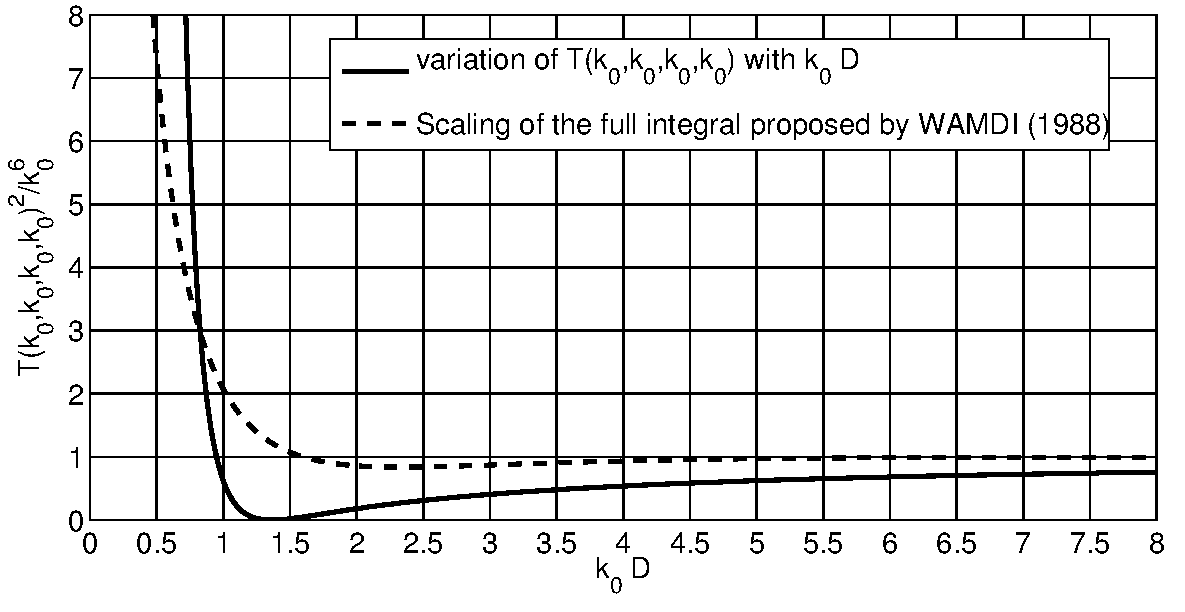
\includegraphics[width=0.70\textwidth]{FIGURES/Tsquared_kD.pdf}}
%\vspace{3.64in}
\caption{Change of the 4-wave coupling coefficient $T$ for equal wavenumbers  $k_1=k_2=k_3=k_4$ as a function of the non-dimensional depth $kD$. The dashed line is the parameterization proposed by the WAMDI Group(1988), and the solid line is the result by Janssen and Onorato (2007).} \label{T2_Snl_vs_KD}
\end{figure}
%%%%%%%%%%%%%%%%%%%%%%%%%%%%%%%%%%%%%%%%%%%%%%%%%%%%%%%%%%%%% end of figure
